\chapter{Background}
\renewcommand{\headrulewidth}{0pt}
\lhead[\thepage]{\leftmark}
\rhead[\leftmark]{\thepage}
\cfoot[]{}

\section{Air pollution}
\subsubsection{Introduction}

Air pollution stands as a critical environmental issue, significantly impacting human health, ecosystems, and climate patterns. According to the World Health Organization (WHO) in 2020, approximately seven million deaths worldwide were attributed to air pollution \citep{who2020world}. Air pollutants such as nitrogen oxides (NOx = NO + NO2), carbon monoxide (CO), ground-level ozone (O3), sulfur dioxide (SO2) and particulate matter (PM), are directly emitted from natural or anthropogenic activities or through atmospheric photochemical reactions. Some of these pollutants are emitted alongside carbon dioxide (CO2) through combustion processes, while others are also short-lived climate forcer having direct or indirect effects on climate change by modulating global radiation budget \citep{RN3}. In addition, ozone can detrimentally impact crop yield, potentially posing future challenges to food security \citep{avnery2011global, avnery2011global2, chuwah2015global, tai2017impacts}.\par
Nitrogen dioxide (NO2) emerges as a particularly concerning pollutant due to its adverse effects on human health \citep{hamra2015lung}. Short-term exposure to elevated NO2 concentrations can cause airway inflammation, increased susceptibility to respiratory infections and allergies, and aggravate existing lung or heart conditions \citep{bono2016air, kelly2011air}. Moreover, NOx lead to environmental changes by altering soil chemistry and biodiversity through nitrogen deposition via dry and wet processes \citep{bobbink2010global}. Additionally, NOx serves as a crucial precursor to tropospheric ozone (O3), along with volatile organic compounds (VOCs) \citep{akimoto2022rethinking}. NOx, CO and non-methane volatile organic compounds (NMVOCs) have an influence on the methane (CH4) lifetime by affecting the atmospheric mixing ratio of hydroxyl radicals (OH) \citep{akimoto2022rethinking}, which act as a primary sink for CH4 \citep{turner2019interpreting}. Both O3 and CH4 are short-lived climate pollutants (SLCPs) that contribute to positive radiative forcing, thereby intensifying global warming \citep{akimoto2022rethinking}. 
Global NOx emissions predominantly stem from fossil fuel combustion within energy, industry and transportation sectors. In 2017, nearly 60\% of global NOx emissions were attributed to the energy generation (22\%), industry (15\%), and on-road transportation (23\%) sectors. These sectors notably contributed to emissions from coal combustion, especially in the energy and industry sectors (accounting for over 46\% of the emissions). Additionally, emissions from the combined combustion of liquid fuels (oil) and natural gas constituted 100\% of on-road NOx emissions \citep{mcduffie2020global}. Considering historical emissions from 1970 to 2017 recorded in the CEDS database  \citep{mcduffie2020global}, global NOx emissions reached their peak between 2011 and 2013, followed by a subsequent 7\% decrease by 2017. This reduction was primarily due to stricter emission standards phased in across North America and Europe since 1992 and in China since 2013 \citep{mcduffie2020global, zheng2018trends}. However, during the same period, global NOx emissions from the energy and industry sectors increased significantly, almost six-fold between 1970 and 2011. This surge was largely driven by regional increments in China, India, the Other Asia/Pacific region, and several African countries. The subsequent decline in emissions between 2011 and 2017 was primarily due to stringent emission control policies in China, particularly targeting coal-fired power plants and industrial coal use \citep{zheng2018trends, liu2015reduced}. Additionally, global emissions of NOx from waste combustion and agricultural activities rose by 2\% and 65\%, respectively, between 1970 and 2017. These increments contributed significantly to offsetting the recent reductions in emissions from regulated combustion sources \citep{mcduffie2020global}. \par

\subsubsection{Impact of weather variations on air pollution changes}

Air pollution is not solely determined by emissions but also by meteorological conditions. The lifetime of NO2 is strongly influenced by meteorological parameters and photochemical reactions \citep{barre2021estimating} and varies seasonally \citep{dragomir2015modeling,kendrick2015diurnal}. During winter, photochemical reaction activity is reduced, resulting in a longer lifetime of the NO2. Additionally, seasonal variations in NO2 concentration are controlled by dispersion processes which are significantly affected by changes in boundary layer height (BLH), wind speed and direction patterns due to temperature inversions in summer and winter \citep{barre2021estimating,kendrick2015diurnal}. Furthermore, seasonal variations of ozone are also influenced by meteorological conditions. The study in China showed that research conducted in China highlighted the seasonal dependence of maximum daily O3 concentrations on ambient temperature rather than solar radiation during spring and summer. Conversely, autumn and winter witnessed solar radiation playing a more crucial role in determining O3 levels. Wind speed exhibited a weak negative correlation with atmospheric O3 levels in spring, summer, and autumn but a weak positive correlation in winter. Moisture levels in spring and autumn also impact O3 concentrations due to the compensation between water vapor and O3. Higher humidity levels stimulate OH radical, elevating O3 concentration in the areas with high NOx. Simultaneously, increased water vapor leads to the consumption of excited oxygen atoms, intensifying O3 loss \citep{yu2021review}. \par
Over the years, Japan has implemented comprehensive measures targeting emissions from both stationary and mobile sources, leading to substantial improvements in air quality since the 1950s. examining air pollution trends from 1970 to 2018 in Japan has shed light on the interplay between these measures and pollution levels \citep{ito202130, kannari2013thirty, wakamatsu2013air}. Findings from these studies have underscored a consistent decline in the concentrations of PM2.5, NO2 and SO2, indicating the direct effectiveness of human-induced emission control strategies in mitigating pollution levels. This reduction in pollutant concentrations aligns with specific actions taken to address emissions. For instance, the decline in nitrogen oxides (NOx) might be attributed to the implementation of stricter regulations governing vehicle emissions. Similarly, the reduction in sulfur dioxide (SO2) levels could be linked to the widespread adoption of marine fuels with lower sulfur content, emphasizing the direct impact of targeted interventions on pollution reduction. Nevertheless, there has been a consistent year-on-year rise in ozone concentrations across extensive areas in Japan, encompassing even rural zones unaffected by direct anthropogenic sources of air pollutants \citep{ito202130}. Previous studies highlighted the significant influence of meteorological fluctuations on ozone levels in Japan. For instance, \citep{kurokawa2009influence} highlighted the sensitivity of springtime ozone variation in Japan to outflows from continental Asia. Additionally, they found a correlation between springtime ozone and the El Nino-Southern Oscillation, indicating a relationship where higher and lower springtime ozone levels are linked to La Nina and El Nino, respectively. The summer of 2019 witnessed widespread occurrences of elevated ozone concentrations throughout Japan, as reported by \citep{fukunaga2021relationship, ito202130}.\citep{fukunaga2021relationship} proposed that the conducive conditions for elevated ozone levels during this time were attributed to clear skies and higher temperatures. They suggested that a migrating anticyclone might have carried ozone and its precursors eastward, contributing to this phenomenon. This emphasizes the importance of not only exploring the direct impact of air pollution control measures but also comprehending the role of meteorological conditions in shaping air pollution dynamics. Investigating these interdependencies could significantly enhance our ability to devise more effective measures to mitigate air pollution effectively. \par

\section{Greenhouse gas}
\subsubsection{Fossil fuel GHG}

Greenhouse gases (GHGs) are atmospheric gases that trap heat and contribute to warming the Earth. The major ones include carbon dioxide (CO2), methane (CH4), nitrous oxide (N2O) and Fluorinated gases (F-gases) like hydrofluorocarbons (HFCs), perfluorocarbons (PFCs), and sulfur hexafluoride (SF6). These gases persist in the atmosphere for various durations, ranging from a few years to thousands of years. They reach a well-mixed state, meaning their concentrations worldwide remain relatively consistent regardless of their sources. These gases differ significantly in their impact on atmospheric warming. To compare their effects, a metric called Global Warming Potential (GWP) was established. GWP measures how much energy emissions of a specific gas, compared to emissions of 1 ton of carbon dioxide, absorb over a given period such as 20, 100, and 500 years. A higher GWP indicates a stronger warming effect on Earth relative to carbon dioxide during that time frame. This standardized unit enables the aggregation of emissions estimates for different gases (e.g., in national GHG inventories) and assists policymakers in evaluating reduction opportunities across sectors and gases. Expressed as ‘CO2 equivalent’ (CO2-e), GWP converts a gas's impact into equivalent tonnes of carbon dioxide. For instance, methane's GWP over 100 years is 27 – 29.8, signifying that one tonne of methane has a warming effect equivalent to 27 – 29.8 tonnes of CO2 over a 100-year period. Furthermore, nitrous oxide (N2O) has the highest impact with GWP over 100 years is 273 \citep{RN3}. However, the amount of nitrous oxide and methane emissions have been less than that of carbon dioxide emission. \par
GHGs originate from diverse sources, encompassing both natural processes and human activities. Carbon dioxide is naturally present in the atmosphere as part of the Earth's carbon cycle, which is consistently exchanged carbon among the atmosphere, oceans, soil, plants, and animals. Human activities are altering the carbon cycle–both by adding more carbon dioxide to the atmosphere and by influencing the ability of natural sinks, like forests and soils, to remove and store carbon dioxide from the atmosphere. While carbon dioxide emissions originate from various natural sources, human-induced emissions have been primarily responsible for the substantial increase in GHGs in the atmosphere since the Industrial Revolution commenced around 1750 \citep{RN3}. In 2019, emissions included approximately 45 ± 5.5 GtCO2 emissions, 11 ± 3.2 GtCO2-eq of methane (CH4), 2.7 ± 1.6 GtCO2-eq of nitrous oxide (N2O) and 1.4 ± 0.41 GtCO2-eq of fluorinated gases (F-gases) (IPCC, 2022). The primary source of carbon dioxide stems from the combustion of fossil fuels within energy conversion systems like boilers in electric power plants, engines in aircraft and automobiles, and in cooking and heating within homes and businesses, accounting for approximately 64\% of emissions. Fossil fuels also play a significant role in methane emissions, the second-largest contributor to global warming. While most GHGs originate from fossil fuel combustion, about one quarter comes from land-related activities like agriculture (mainly methane and nitrous oxide) and deforestation (mainly carbon dioxide). Additional emissions come from industrial processes (primarily carbon dioxide, nitrous oxide, and F-gases), as well as municipal waste and wastewater (mainly CH4) (IPCC, 2022). 
The estimated global net anthropogenic GHGs emissions for the year 2019 reached approximately 59 ± 6.6 GtCO2-eq, marking a 12\% increase compared to the levels seen in 2010 and a significant 54\% surge compared to the figures from 1990. Among these emissions, the dominant share and escalating growth came from CO2 emissions originating from fossil fuels combustion and industrial processes (CO2-FFI), followed closely by methane emissions. Notably, the highest relative growth occurred in F-gases, albeit starting from minimal levels in 1990. During 2010–2019 period, the average annual GHG emissions surpassed those of any preceding decade on record. However, the rate of growth between 2010 and 2019 (1.3\% yr-1) was comparatively lower than that observed between 2000 and 2009 (2.1\% yr-1). In 2019, a substantial 79\% of global GHG emissions stemmed from energy, industry, transport, and building sectors combined, while 22\% originated from agriculture, forestry, and other land use (AFOLU). Global gross domestic product (GDP) per capita and population growth remained the primary drivers of CO2 emissions from fossil fuel combustion throughout the last decade. The trends from 1990 continued through the years 2010-2019, with GDP per capita and population growth contributing to emissions escalation by 2.3\% yr–1 and 1.2\% yr–1, respectively. This growth outpaced the reduction in the use of energy per unit of GDP (–2\% yr –1, globally) as well as improvements in the carbon intensity of energy (–0.3\% yr –1). Therefore, emissions reductions in CO2-FFI due to improvements in energy intensity of GDP and carbon intensity of energy, have been less than emissions increase from rising global activity levels in industry, energy supply, transport, agriculture and buildings (IPCC, 2022). \par

\subsubsection{Terrestrial carbon fluxes}

Terrestrial ecosystems play a crucial role in mitigating global warming by serving as a persistent carbon sink, actively absorbing and storing excess carbon dioxide from the atmosphere \citep{pan2011large}. Over the period from 2010 to 2019, the terrestrial CO2 sink is estimated to offset fossil CO2 emissions by 35\%, surpassing the ocean, which is projected to remove 26\% of fossil-fuel-derived CO2 \citep{friedlingstein2020global, wang2022disentangling}. The substantial global carbon flux, known as terrestrial gross primary production (GPP), significantly contributes to the reduction of anthropogenic CO2 emissions \citep{beer2010terrestrial}. \par

\begin{figure}
    \centering
    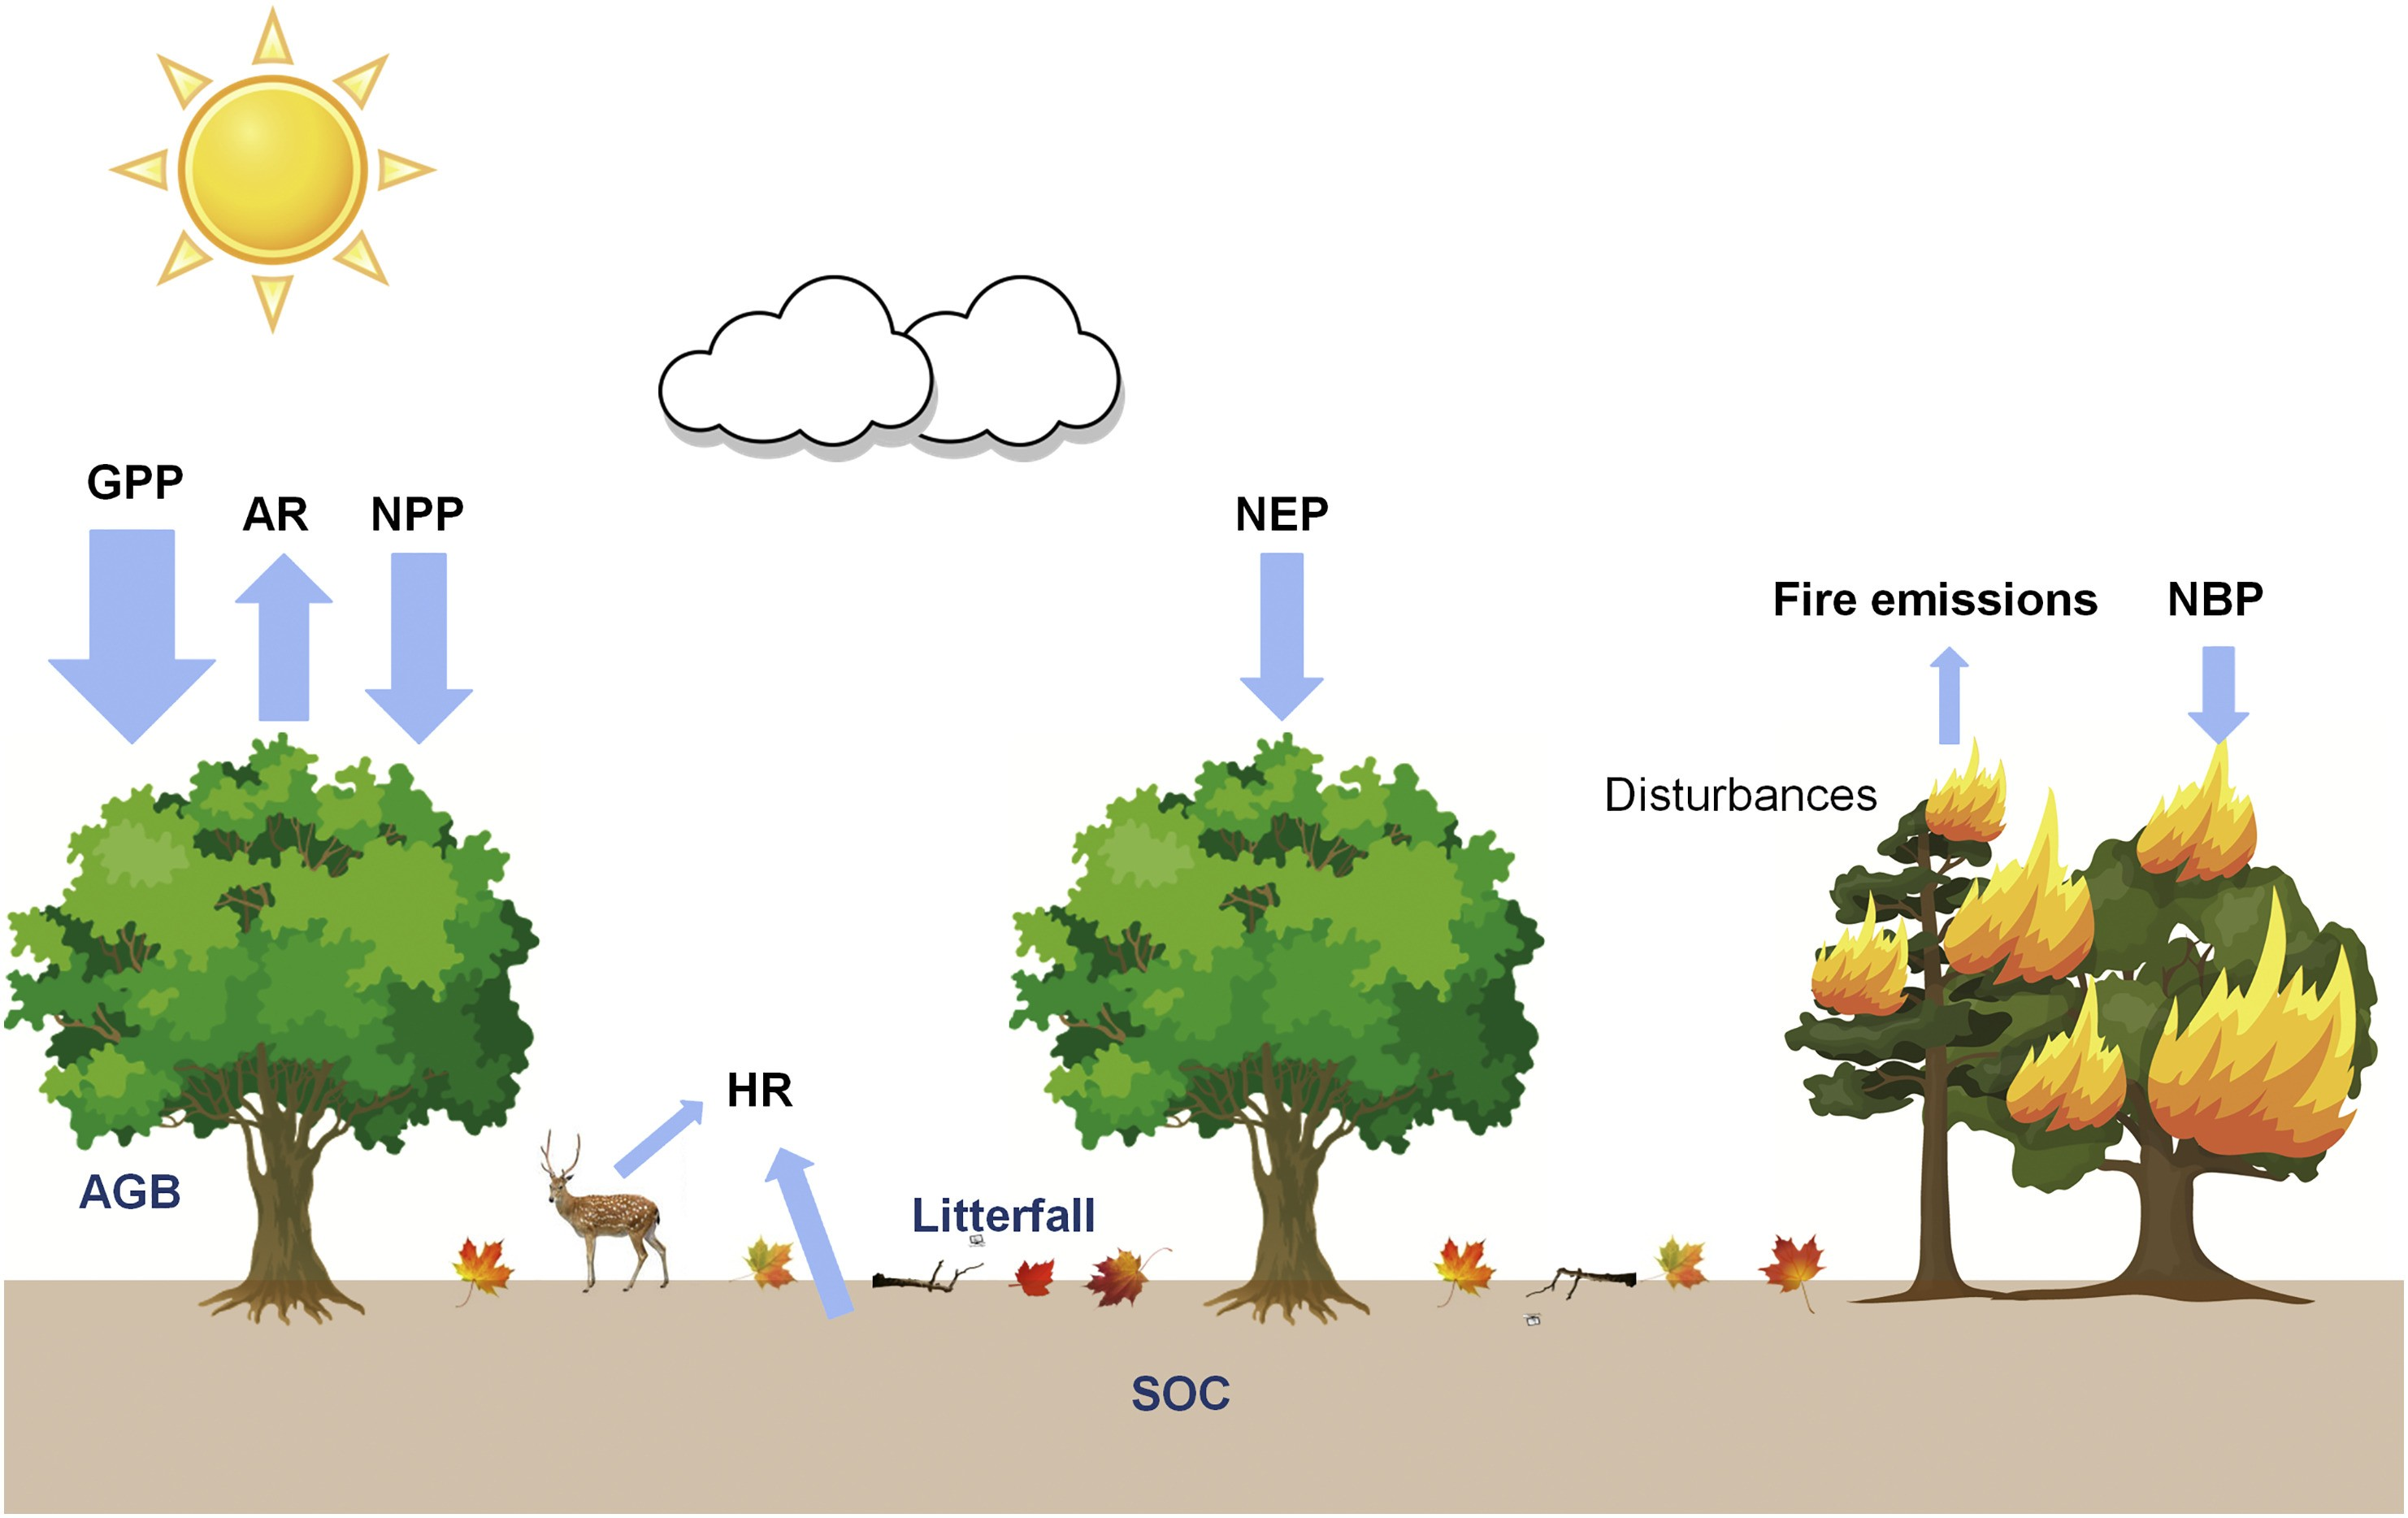
\includegraphics[width=\textwidth]{figs/chap2/fig1.jpg}
    \caption{Terrestrial carbon cycle \citep{xiao2019remote}}
    \label{chap2:fig_fig1}
\end{figure}

% need recheck
As illustrated in Figure \ref{chap2:fig_fig1}, we illustrate that Gross Primary Production (GPP) represents the total carbon sequestered by terrestrial ecosystems, serving as the foundation for food, wood, and fiber production and thereby holding significant implications for human well-being \citep{xiao2019remote}. A portion of the absorbed carbon is released back into the atmosphere through plant autotrophic respiration (AR). The disparity between GPP and AR is denoted as Net Primary Production (NPP). The material that falls to the ground from plants, such as leaves, branches, flowers, and fruits, known as litterfall, contributes to the accumulation of soil organic carbon (SOC). The size of the SOC pool is influenced by carbon inputs from litterfall and root mortality/exudation, as well as carbon release from decomposition, termed heterotrophic respiration (HR) \citep{liu2011simulating}. AR and HR collectively constitute ecosystem respiration (RECO). Net Ecosystem Production (NEP) is the absolute difference between GPP and RECO. Processes like deforestation, harvesting, and fires can result in carbon loss, with the net ecosystem carbon balance referred to as Net Biome Production (NBP). Disturbances, crucial ecosystem processes, impact carbon cycle dynamics. Wildfires, for example, lead to immediate carbon transfer from ecosystems to the atmosphere. Fires, along with other disturbances such as insect and disease outbreaks, droughts, severe storms, and harvesting, can cause substantial effects on GPP and respiration, with these impacts persisting for decades as ecosystems recover. \par

Estimating GPP involves various methods, such as simulating dynamic global vegetation models (DGVMs) like those employed in the TRENDY project \citep{sitch2015recent, le2018global}, upscaling from measurements obtained through eddy covariance (EC) flux tower and satellite observations \citep{jung2019fluxcom, zeng2020global}. However, all these approaches rely on plant functional types (PFTs) to estimate ecosystem productivity \citep{poulter2011plant, poulter2015plant, lin2021improved, guo2023estimating, yan2023integrating}. Inconsistencies in PFT maps can significantly contribute to uncertainties in GPP estimations, as well as other climate-relevant variables, at both regional and global scales \citep{poulter2011plant}. Particularly in the tropical region, the sparse distribution of EC sites, the high species richness of trees, and the complex vertical structure of tropical rainforests pose challenges \citep{montgomery2001forest}, making it difficult to accurately quantify the seasonality of carbon fluxes \citep{xu2015satellite}. \par

\section{Relationship between air pollution and greenhouse gas}
NO2 possesses the potential to serve as an indicator for monitoring localized fossil fuel CO2 emissions owing to its short lifetime in the atmosphere and significant signal compared to CO2 \citep{miyazaki2023predictability}.\par
\section{Air pollution, GHGs and SDGs}

To slowdown the climate warming, immediate reductions of GHGs and “neutral carbon” is effective way to achieve the goal of 1.5 degree Celsius by 2050 has been proposed by IPCC…. The most effective way to reduce CO2 emissions is to reduce fossil fuel consumption. Many strategies for reducing CO2 emissions from energy are cross-cutting and apply to homes, businesses, industry, and transportation. Additionally, land-based mitigation measures including afforestation, reforestation, improvement of soils, and other activities to enhance the capacity of CO2 removal from the atmosphere. The impacts of such mitigation actions go far beyond the goal of climate action (SDG 13) and life on land (SDG 15) and contribute to meeting 15 other SDGs. Such mitigation actions bring health gains through improved air quality, and have positive significant macro- and micro-economic effects, such as increased productivity of labour, job creation, reduced poverty, especially energy poverty, and improved energy security. \par

